\section{Beacon Server}
The \TDC \BS starts PCB propagation to construct a (half) path from \TDC to \STUB \ADs. The \BS specifies the packet type as PCB in the header (viz., Figure~\ref{fig:hdr-common}), puts its own opaque fields in the packet, and forwards it to customer \ADs. The \BS can specify the next hop \AD (to which it would send PCB) using the egress interface ID since egress interface to \AD mapping is available in the topology file. The ingress routers of an \AD, once they receive a PCB from their provider \AD, forward the PCB to the local \BS; and the local \BS adds its AID and opaque field to the PCB. Every border routers know the \BS location (i.e., address or AID), hence they fill the Destination AID field with the address of the \BS and forward the PCB. The \BS queues all PCBs arrived for a pre-defined time interval (denoted by $T_Q$), choose $k$ PCBs per customer \AD, add its own marking, and propagate them to the chosen \ADs. This PCB propagation ends at \STUB \ADs. We describe how a \BS handles PCBs in detail below.

\begin{figure*}[ht]
\centering
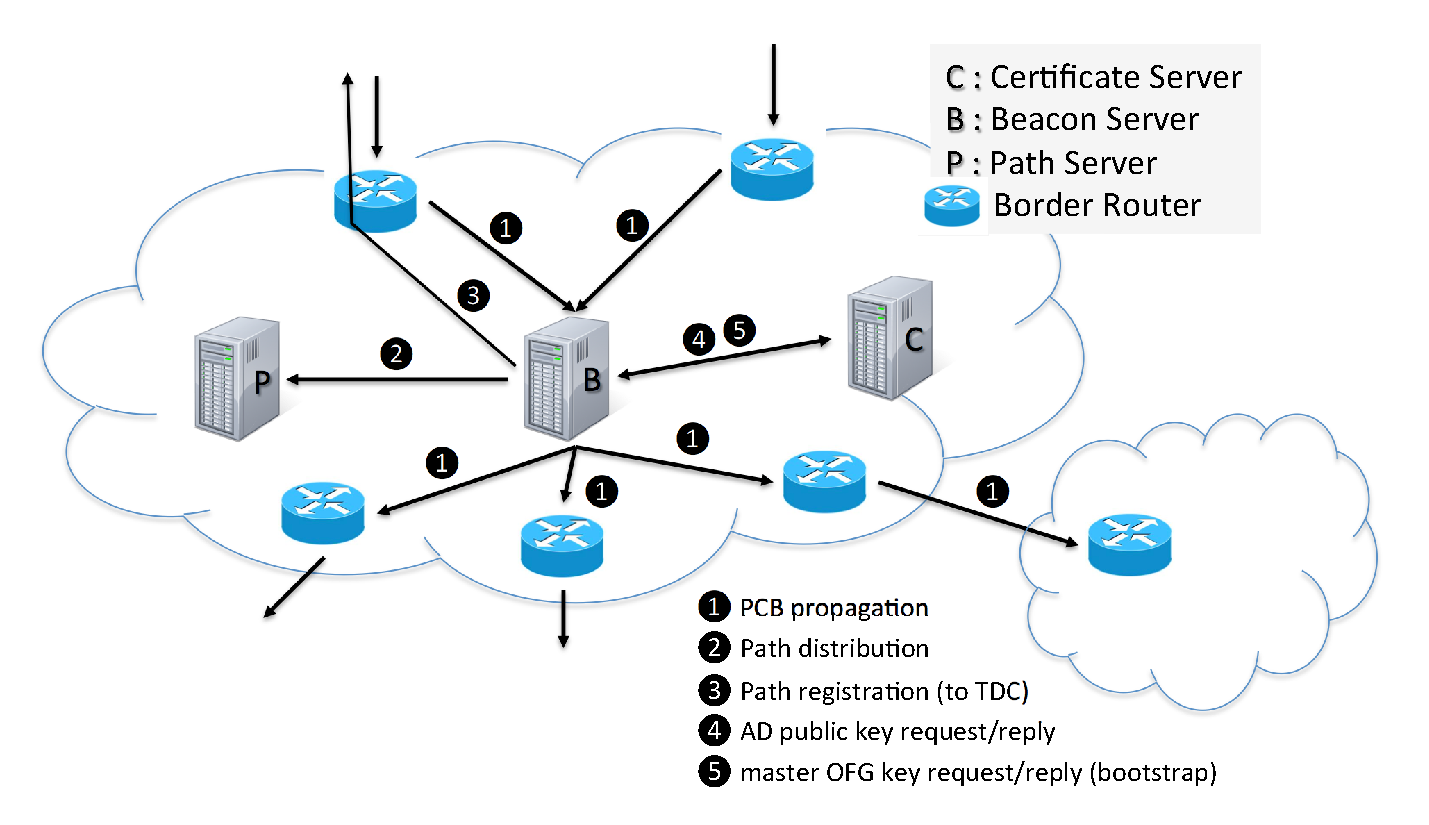
\includegraphics[width=.9\columnwidth]{./fig/bs_message.eps}
\caption{Beacon Server messages.}\label{fig:bs-message}
\end{figure*}

\subsection{Opaque Field Generation}
For path freshness, a \BS generates the opaque field by hashing the current timestamp and expiration time (EXP) with the ingress and egress interfaces. As a result, the opaque fields created with at different timestamps are different even if they have the same ingress-egress interface pair. Furthermore, to limit the path (i.e., opaque field) lifetime, \BSs set the EXP field in the header (viz., Figure~\ref{fig:hdr-common}) to one of four types (i.e., 6, 12, 18, 24 hours) based on their local policy. Since all border routers know the current and previous OFG keys, they can compute the opaque field for a specific timestamp and hence verify the opaque field carried in a data packet (that was originally generated by the \BS). We note that every data packet carries the timestamp and expiration in its header. %Once a border router receives a OFG key, the router stores the key in its {\bf Key Table} so as to reuse that key (without hash computation) for verifying other packets carrying the same timestamp.

{\bf Key management:} Key revocation and recovery after failures or compromise. \soobum{Key recovery seems not an issue, yet revocation needs to be preceded by identification of key compromise}

\subsection{PCB Selection/Propagation}~\label{subsec:pcb_selection}
The \BS queues PCBs for a predefined PCB propagation period (e.g., 10
seconds), and selects $k$ PCBs to propagate to customer \ADs, each of
which may have a different set of selection policies. We consider two
classes of policies: (1) exclusion and (2) prioritization. Exclusion
policies specify paths that should be avoid, and prioritization
policies specify the preference between paths.

The current implementation supports four exclusion policies that we
believe are commonly used:
\begin{itemize}
\item {\bf Maximum age ($A_{max}$, in seconds)}: The age of a PCB is
  defined as the length of time that the PCB has existed. This policy
  excludes paths with age above $A_{max}$.
\item {\bf Maximum path length ($L_{max}$, in hops)}: This policy
  excludes paths above $L_{max}$ AD-level hops.
\item {\bf Minimum elapsed time since last propagation ($E_{min}$, in
  seconds)}: While we flexibly allow re-propagation of the same PCB
  (for reasons like improving fault tolerance), we also would like to
  maintain a good level of path diversity by not propagating the same
  PCB over and over again in a short period of time. Hence, this
  policy excludes paths that have been propagated in last $E_{min}$
  time.
\item {\bf Unwanted ADs:} This policy allows exclusion of paths
  containing certain ADs. For example, the administrator may want to
  avoid going through ADs that are identified to be malicious or
  provide low quality services.
\end{itemize}

The rest of the PCBs are prioritized based on their {\bf Path
  Fidelity}, a metric defined in terms of age, path length, and path
freshness. We would like to incorporate other parameters such as
local desirability, available bandwidth, and disjointness in the
future. 


%% PCB selection is determined using {\bf Path Fidelity} defined in terms
%% of local desirability, path length, path freshness, and available
%% bandwidth.

\begin{itemize}
\item {\bf Age ($A_p$):} As defined earlier, the age of a PCB is the
  length of time that the PCB has existed.
\item {\bf Path length ($L_p$):} \AD-level path length to \TDC. The
  path length is the most {\em stable} and {\em reliable} estimate for
  path quality.
\item {\bf Path freshness ($E_p$):} time elapsed since a path's last
  propagation. Non-propagated paths for a while would have higher
  freshness and hence have chance to be selected; e.g., a maximally
  disjoint path from previous propagations would be selected with
  higher probability.
\item {\bf Local desirability ($D_p$):} a value ranging from 0 to 1,
  where 1 indicates the highest desirability. An \AD decides a path's
  local desirability based on the contracts with provider and customer
  \ADs or to optimize its local network resource (e.g., local traffic
  engineering).
\item {\bf Available bandwidth ($B_p$):} available bandwidth would be
  the most accurate measure of path quality if long-term (e.g., hours
  rather than seconds), static bandwidth allocation can be made.
\item {\bf Path disjointness:} how much the current path differs from
  all previous selections. We can quantify the path disjointness by
  the number of new ADs the current PCB covers.
\end{itemize}

In the current implementation, the prioritization policies specify the
weights ($w_1$, $w_2$, and $w_3$) of each term in computing path
fidelity:
\[
F_p = 1 - (w_1 \cdot \frac{A_p}{A_{max}} + w_2 \cdot \frac{L_p}{L_{max}} + w_3 \cdot \frac{E_{min}}{E_{p}})
\]
Note that when $w_1 + w_2 + w_3 = 1$, $F_p$ is between 0 and 1.

%% The path fidelity, denoted by $F_p$, is defined in terms of the above metrics.
%% \[
%% F_p = w_1 \cdot D_p + w_2 \cdot \frac{L_{MIN}}{L_p} + w_3 \cdot \frac{E_p}{E_{MAX}} + w_4 \cdot \frac{B_p}{B_{MAX}}
%% \]
%% where $L_{MIN}$, $E_{MAX}$, and $B_{MAX}$ are the minimum path length,
%% maximum freshness, and the maximum available bandwidth
%% respectively. 

The \BS distinguish a path by a series of tuples, namely AID, ingress
interface and egress interface, marked by each \AD. Newly arrived PCBs
are added to a {\em beacon table}, and the \BS maintains the size of
the beacon table by removing oldest PCBs (PCBs with smallest
timestamps).  \note{HC: the current implementation doesn't seem to
  detect duplications...}  Periodically, the \BS initiates the path
selection process as follows. For each customer \AD, the \BS
prioritizes and filters PCBs in the beacon table according to this
\AD's policies, propagates to the \AD $k$ PCBs with the highest
priority, and keeps track of what PCBs have been propagated. The \BS
can also select paths in a probabilistic fashion: instead of selecting
the top-$k$ paths, the \BS scans paths from the highest priority to
the lowest, and selects each path with a certain probability until $k$
paths are selected.


%% When a new PCB arrives, the \BS queues the PCB in its local buffer
%% after checking duplicate and assigning a local timestamp (as
%% opposed to the global timestamp marked by \TDC) to the PCB. If the
%% \BS cannot find a duplicate path in its PCB queue, it assigns a
%% current local timestamp to the PCB, which would be used for
%% computing path freshness. If the \BS find a duplicate, it copies
%% the old (duplicate) PCB's local timestamp to the new PCB and
%% replaces the old PCB with the new one. That is, for each path, the
%% \BS only keeps the most recently arrived PCB while keeping track of
%% the age of the path (i.e., how long the path was kept in the queue
%% without being propagated). The \BS controls the diversity of
%% propagated paths by adjusting $A_{max}$: e.g., a lower $E_{MAX}$
%% would increase the path diversity.  The \BS selects a PCB from its
%% PCB queue with a probability proportional to the path fidelity
%% computed by the above equation.

%\soobum{More details on path selection algorithm need to be described and analyzed}


\subsection{Path Registration/Distribution}
An \AD's \BS selects $k$ paths from all received PCBs in order to provide remote source \ADs with down-paths and help those \ADs to establish end-to-end paths. To this end, the \BS registers the selected paths to the \TDC \PS. The \BS does not need to register $k$ paths at a time, yet can register paths whenever it wants to do. However, the number of total registered paths at the \TDC \PS cannot exceed $k$. The path registration request should be signed by the requesting \AD to prevent any forgery by malicious \ADs. The \TDC \PS, on receiving a path registration request, verifies the signature and registers the path as: if the \PS has less than $k$ registered paths for the \AD, it registers the path; otherwise the \PS replaces the oldest path (that has the smallest timestamp) with the new one. The \PS limits the number of \AD's path registrations to prevent malicious \ADs from overloading the \TDC \PS and from exploiting too many paths (for attack purposes).

The \BS informs $k$ registered paths to local \PS(s) so that these paths can be used as up-paths to \TDC. Note that the local \PS provides $k$ up-paths to endhosts. Furthermore, the \BS provides some of non-registered paths to the local \PS. These non-registered paths can be used as up-paths as well, yet the packets forwarded along the non-registered paths have low priority than those of registered paths in the presence of congestion. \soobum{need to refer to the SCION DDoS to explain packet priorities}

\begin{comment}
\subsection{Key Table Management}~\label{subsec:key-table-management}
The \BS generates an OFG key by hashing the current timestamp in the PCB (marked by the \TDC \BS) and its own expiration time with the master OFG key; i.e., $K_i(t)$ = $\textrm{H}_{K_i^{master}}(\textrm{timestamp} || \textrm{EXP})$. Since border routers know $K_i^{master}$, they can verify the opaque field carried in a data packet after computing $K_i(t)$. However, the border routers, instead of computing $K_i(t)$ for every packets, keep $K_i(t)$ in their Key Table for up to its expiration time in order to reduce computational overhead. With this, the router would lookup the key table first and if the table contains a stale (i.e., expired) key for the corresponding time, the router compute and store the OFG key. For example, if a PCB is generated in every 1 minute, the routers need to keep at most 1440 $\times$ 4 = 5760 keys, which only requires a small amount of memory (less than 100KB for 128 bit keys) while enabling fast key retrieval from the table (a router determines a key location in the memory using the timestamp and expiration time). \ADs synchronize timestamp using a time server or a satellite time. Time synchronization can be made with low precision if \PSs and border routers allow a sufficient grace period (e.g., several minutes) after a path expires.\soobum{Need to elaborate the time synchronization; e.g., when it's required} 
\end{comment}

\subsection{Bootstrapping}
The \BS has to be prepared with the following information for PCB propagation.
Specifically, the \BS retrieves 
\begin{itemize}
\item the OFG key from the \CS for Opaque Field generation 
\item \AD public keys for PCB verification
\item the topology file from the \CS for PCB propagation
\end{itemize}
The \CS handles all intra- and inter-AD certificate requests and stores the results for all entities within an \AD. Hence, the \BS contacts the \CS to get necessary \AD public keys for signature verification. To reduce the communication overhead during bootstrapping, the \BS starts with local copies of the above data and update them later if necessary. We note that the topology file and \AD public keys not frequently changed (i.e., static), hence they can be stored at the \BS. The \BS reads inter-\AD connectivity information from the topology file and decides how to propagate PCBs. Specifically, the \BS propagates PCBs to the interfaces that connect to customer \ADs (this information is contained in the topology file). Initially, the \BS sets the status of all interfaces registered in the topology file to {\em active} in its local database; yet the \BS changes the status to {\em inactive} for any interface to which propagating a PCB failed. \soobum{A control message protocol (like ICMP) and error messages (or codes) need to be defined.}

\begin{comment}
PCB Propagation
Maintain most recent (Timestamp, Opaque Field Generation Key) acquired 
from Certificate Server (CS)
	Request the pair to CS if it does not have (e.g., due to reboot)
	How often should the OFG Key renew?
Maintain (AID, Public-Key) for PCB signature verification 
	Request the pair to CS if it does not have (first seen AID)
Start Queueing PCBs if a new timestamp arrives – use per child AD queue / verify sign. on arrival
Stop Queueing PCBs if current_time – start_time(of current timestamp) > MAX_PROP_DELAY
Pick k PCBs per child AD based on the preset rules; 
	0. local policy (traffic engineering)
	1. shortest path length
	2. maximally disjoint from previous n propagation
	3. ?
Mark Opaque Field with the present OFG key; H(master OFG key||timestamp)
Propagate k PCBs to children and purge Queue
Add the present OFG key to Key Table (index, the present OFG key)
Multicast all (or selected) Paths to local Path Servers after removing all signatures and adding its own signature (use for best effort paths)
\end{comment}
